\documentclass[a4paper,11pt,english]{article} 

\usepackage[left=1in,right=1in,top=1in,bottom=1in]{geometry}
\usepackage[utf8]{inputenc} 
\usepackage[T1]{fontenc} 
\usepackage[english]{babel}
\usepackage{amsmath,amsthm,amsfonts,amssymb,amstext} 
\usepackage{textcomp}
\usepackage{upgreek} 
\usepackage[final]{graphicx}      
%\usepackage{epstopdf}
%\usepackage{float} 
%\usepackage[font=footnotesize,labelfont=bf,textfont=it]{caption} 
\usepackage[usenames,dvipsnames]{xcolor} 
%\usepackage{pdfpages} 
%\usepackage{siunitx}
%\captionsetup[figure]{name=Fig.} 
%\captionsetup[table]{name=Tab.} 
\usepackage[bookmarks=true,bookmarksnumbered=true]{hyperref}
%\usepackage[round]{natbib}
%\usepackage{smartdiagram}

\parindent 0cm 
\addtolength{\textheight}{0cm}
\addtolength{\voffset}{0cm} 
\setlength{\parskip}{0.6\baselineskip}

\begin{document}

\title{\textbf{The GALAH survey} \\ Update on spectroscpic analysis pipeline}
\author{WG4 - Sven Buder, contributions by Anish Amarsi, Jane Lin, Karin Lind, Thomas Nordlander}

\maketitle

\section{Important changes after GALAH DR2}

\subsection{Spectroscopic synthesis pipeline available for members}

The pectroscopic synthesis pipeline is now open for all GALAH members to use via

\url{https://galah-survey.org/wiki/galah-spectrum-synthesis-pipeline}

\subsection{Documents in preparation of GALAH DR3 available on github}

Initial documents for the preparation of GALAH DR3 have been uploaded on a private (hidden) repository on

\url{https://github.com/svenbuder/GALAH_DR3}

If you want to access to these documents, please email Sven to be added as a collaborator (you need a github account for this).

\subsection{Updates regarding SME}

\begin{itemize}
\item Pipeline finally and successfully converted to the recent SME version 536 (if interested, ask WG4 regarding the major changes). Thanks to Thomas Nordlander!
\item Improved continuum selection and normalisation with SME. Thanks to Karin Lind!
\item Non-LTE now also for H (in addition to Li, O, Na, Mg, Al, Si, and Fe). Thanks to Anish Amarsi!
\end{itemize}

\subsection{Updates regarding use of \textit{Gaia} DR2 and asterseismic data}

\begin{figure}[!ht]
\centering
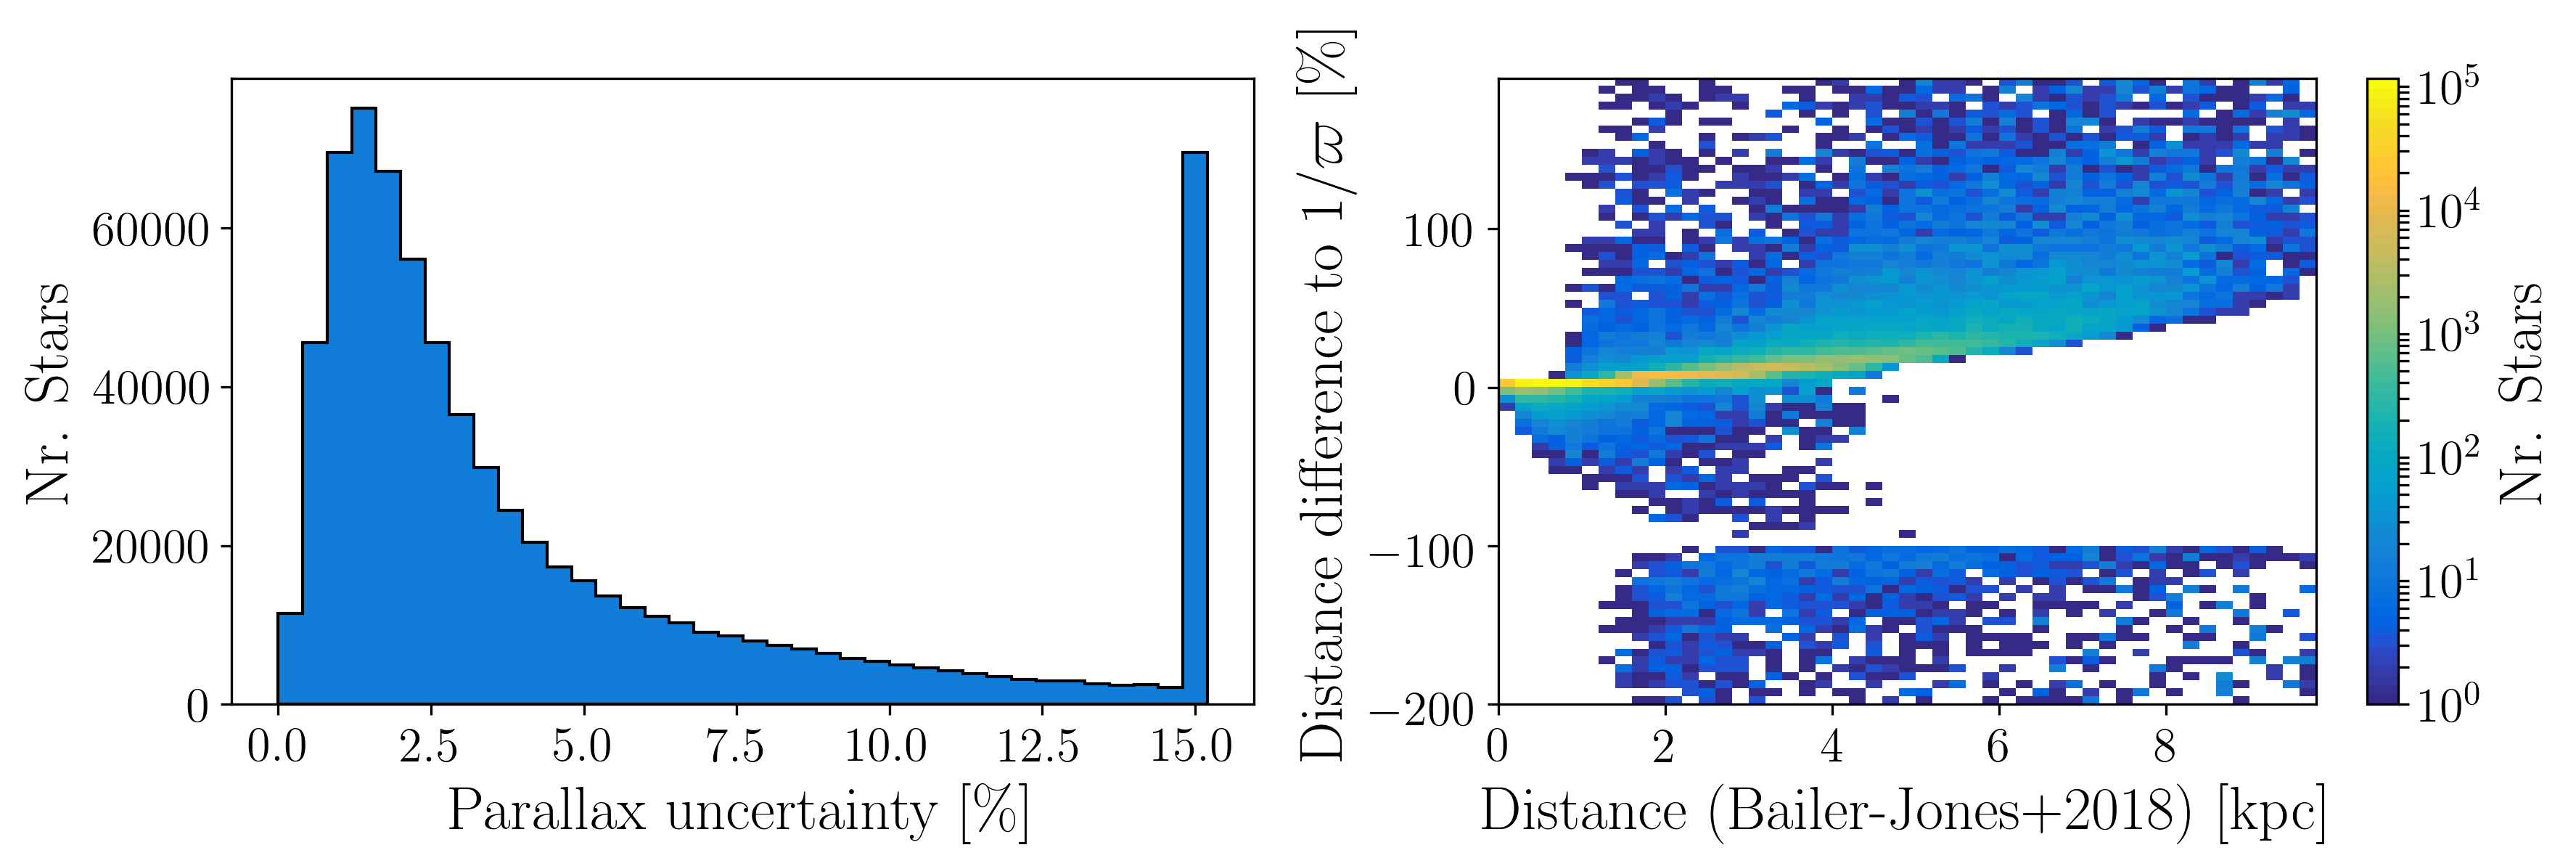
\includegraphics[width=\textwidth]{../../input/figures/parallax_uncertainties.png}
\caption{Overview of parallaxes/distances of the stars observed by GALAH.}
\label{fig:parallax_overview}
\end{figure}

\begin{itemize}
\item Parallaxes now available for almost all stars observed by GALAH and a vast majority of them are very good, see \autoref{fig:parallax_overview}
\item The asteroseismic information provided by Sanjib Sharma and others have been used to run a pipeline version which constrains $\log g$ as a function of $T_\text{eff}$ and $\nu_\text{max}$, which consists of up to 3175 stars (including bad S/N, bad $\nu_text{max}$ values, and bad reductions).
\item For the interim mass and age estimation, we have switched to the use of Parsec isochrones, which include core helium burning stars (in contrary to Dartmouth isochrones) and alpha-enhancement (in contrary to MIST). Thanks to Jane Lin!
\end{itemize}

\section{Performances}

\subsection{\textit{Gaia} FGK benchmark stars}

\autoref{fig:gbs_performance}

\begin{figure}[!ht]
\centering
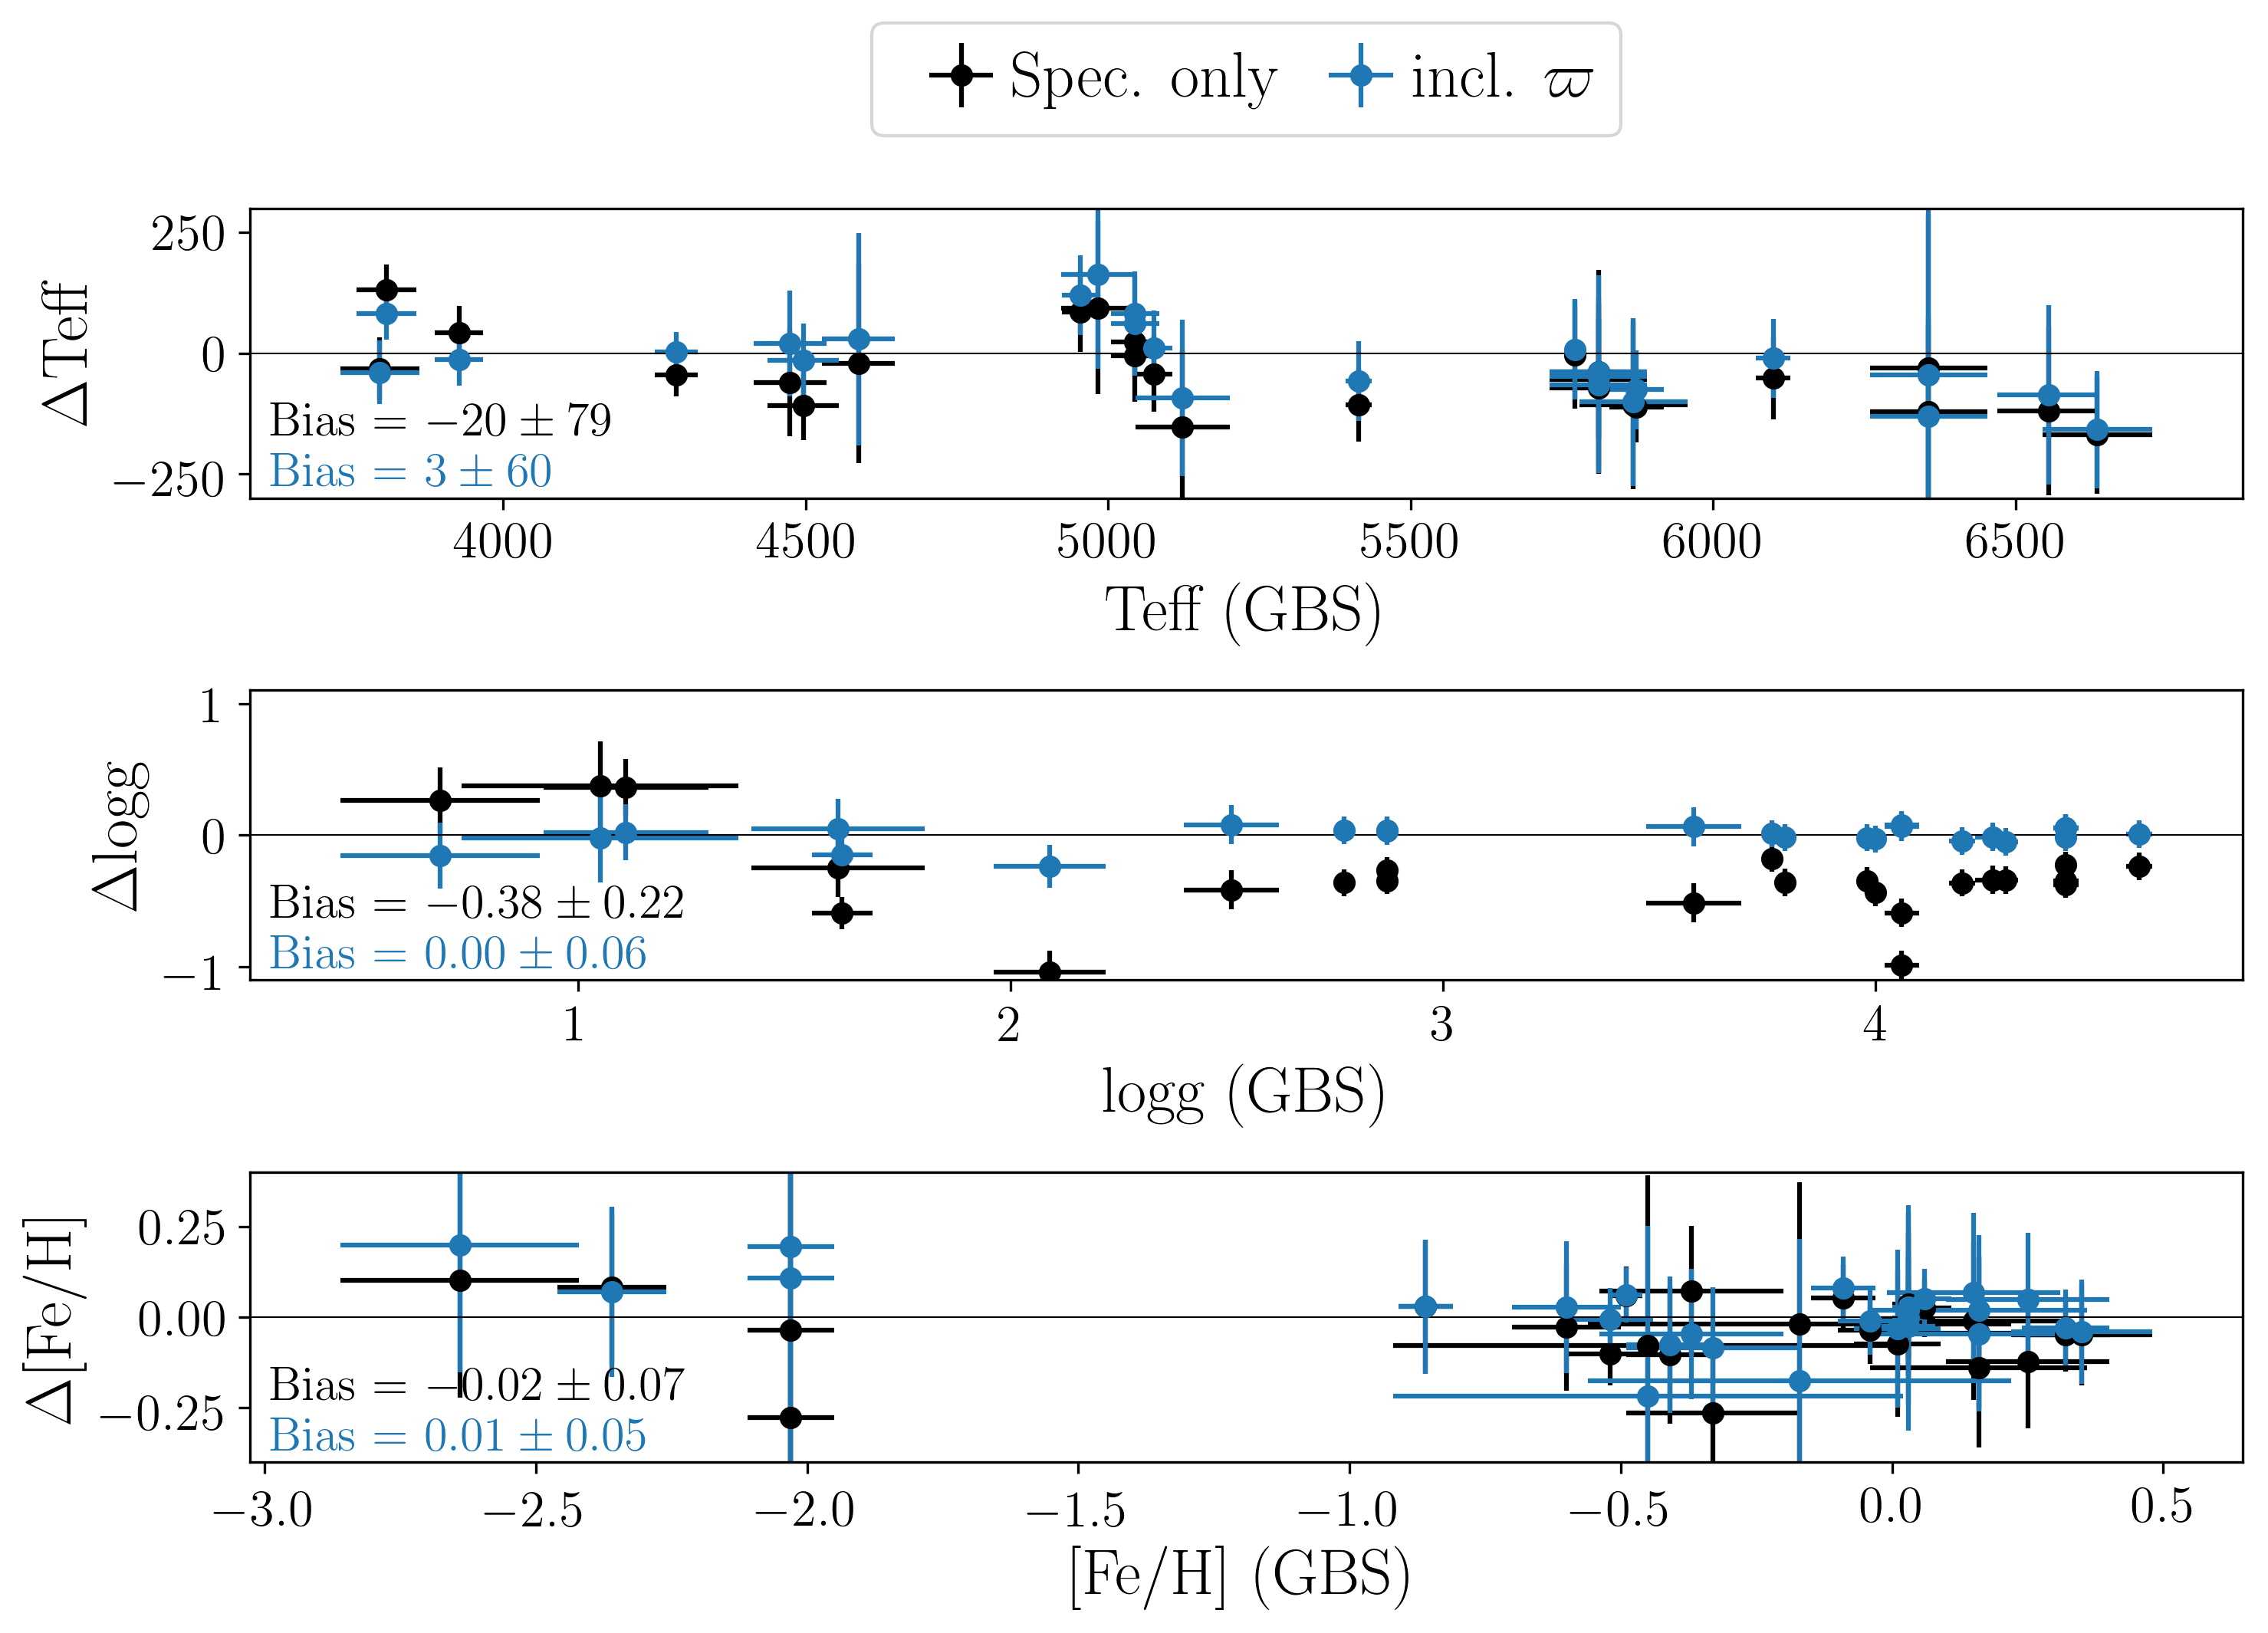
\includegraphics[width=\textwidth]{../../gbs/figures/gbs_performance_free_lbol.png}
\caption{Performance of GALAH synthesis pipeline without (black) and with (blue) bolometric information.}
\label{fig:gbs_performance}
\end{figure}

\subsection{Stars with asteroseismic information}

\subsection{Stars in clusters}

\autoref{fig:cluster_overview}

\begin{figure}[!ht]
\centering
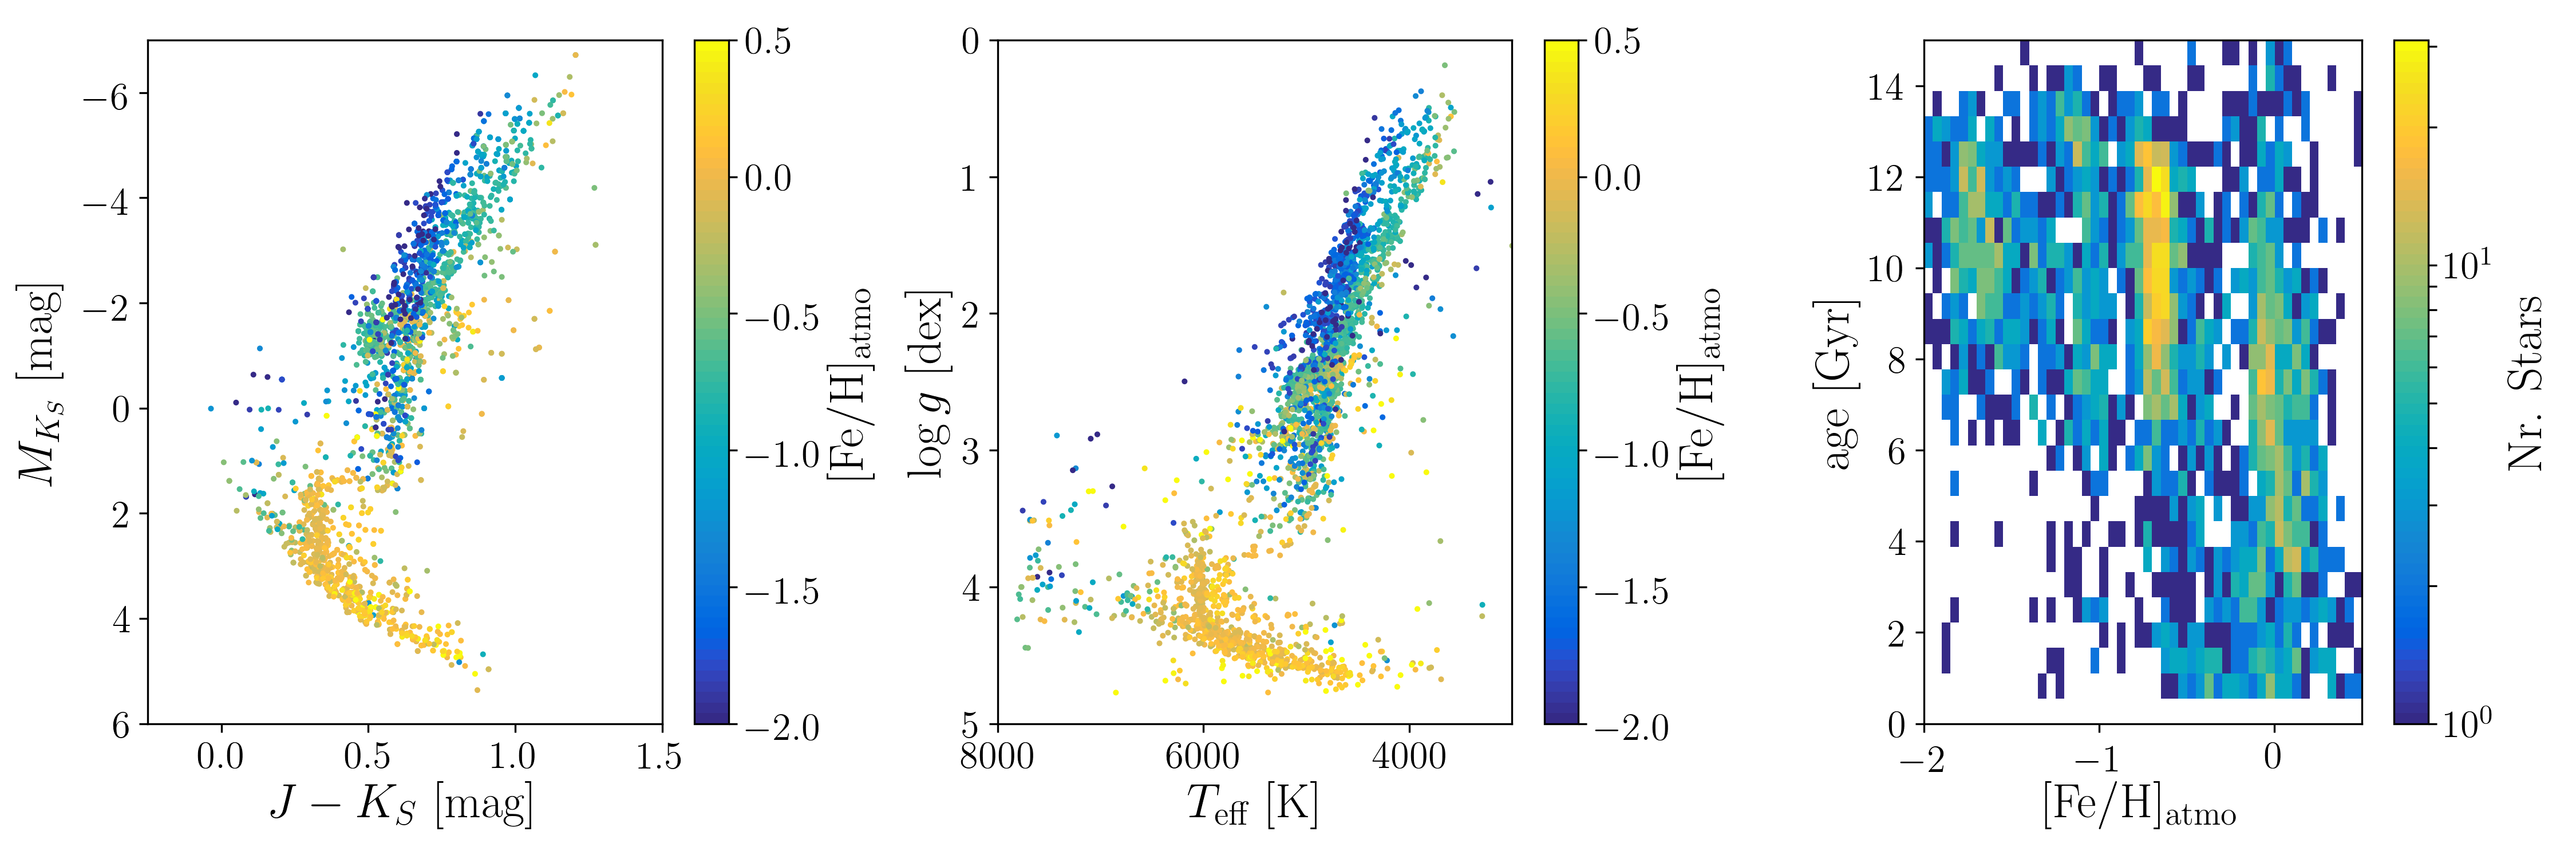
\includegraphics[width=\textwidth]{../../clusters/figures/CMD_Kiel_FehAge.png}
\caption{Overview of cluster stars observed by GALAH.}
\label{fig:cluster_overview}
\end{figure}

\section{Additional information}

\end{document}